%% Use the hmcposter class with the clinic document-class option.
\documentclass[clinic]{hmcposter}
\usepackage{graphicx}
\usepackage{natbib}
\usepackage{booktabs}
\usepackage{subfig}
\usepackage{amsmath}
\usepackage{textcomp}
\usepackage{url}

%% For a Clinic poster, there is no author (the author is the team).

%% Project Year.
%% The year is provided using the \year command.
\posteryear{2019}

%% Project Title.
%% The title of the poster should probably be the name of your
%% Clinic project.
\title{Extracting Educational Priorities\protect\\ for Workforce Innovation}


%% Sponsor's Name.
%% Your sponsoring institution's name.
\sponsor{PilotCity}

%% Sponsor's Logo.
%% The name (base name only; no extension) of an image file with
%% the sponsor's logo.  Ideally, you'll have a PDF version that is
%% resolution-independent.  If not, you'll need a high-resolution
%% PNG file to allow us to print it at a large size without the
%% image becoming blurred.
\sponsorlogo{logo}

%% Optional -- if your sponsor's logo looks too small or too big,
%% you can adjust its width with the \sponsorlogowidth command.
%% (The height of the logo image is automatically adjusted to
%% preserve the image's aspect ratio.)
%%
%% Note that the argument must be a TeX length; for example, 3in,
%% 5cm, 120pt, etc.  The default width is 2in.
\sponsorlogowidth{4in}


%% Optional -- if your sponsor is hot about their intellectual
%% property and insists on having a copyright statement on the
%% poster, you can use the \copyrightholder command to supply a
%% name for a copyright holder for your poster.
% \copyrightholder{Sponsoring Corporation, Inc.}


%% Define the \BibTeX command, used in our example document.
\providecommand{\bibtex}{{\rmfamily B\kern-.05em%
    \textsc{i\kern-.025em b}\kern-.08em%
    T\kern-.1667em\lower.7ex\hbox{E}\kern-.125emX}}


\pagestyle{fancy}

\begin{document}

\begin{poster}

\section{Stakeholders}

\begin{multicols}{2}
\centering
\begin{figure}

\includegraphics[width=150]{pilotcity.png}
\end{figure}
\begin{itemize}
\item Startup in San Leandro, CA
\item Connects classrooms to work-based learning opportunities and internships with global tech companies
\end{itemize}
\vfill
\columnbreak
\centering
\begin{figure}

\includegraphics[width=200]{ies.png}
\end{figure}
\begin{itemize}
\item R\&D branch of the U.S. DoED
\item Extracts data-driven educational insight to inform educators, policy makers, and the public
\end{itemize}
\end{multicols}

\section{Problem Statement}
We were tasked with extracting \textbf{ \textcolor{hmcorange}{{\large educational priorities}}} from \textbf{\textcolor{hmcorange}{{\large uncurated}}} data sources and developing a \textbf{\textcolor{hmcorange}{{\large recommender system}}} to \textbf{\textcolor{hmcorange}{{\large automate}}} PilotCity's program delivery. Further responsibilities included building a \textbf{\textcolor{hmcorange}{{\large web-based application}}} for PilotCity users and a \textbf{\textcolor{hmcorange}{{\large topic modeling engine}}} to gain insight from unstructured data.

\section{Deliverables}

\subsection{Web-Based Application}%

\begin{figure}
  \centering
        \subfloat[][Type of User]{\scalebox{.26}{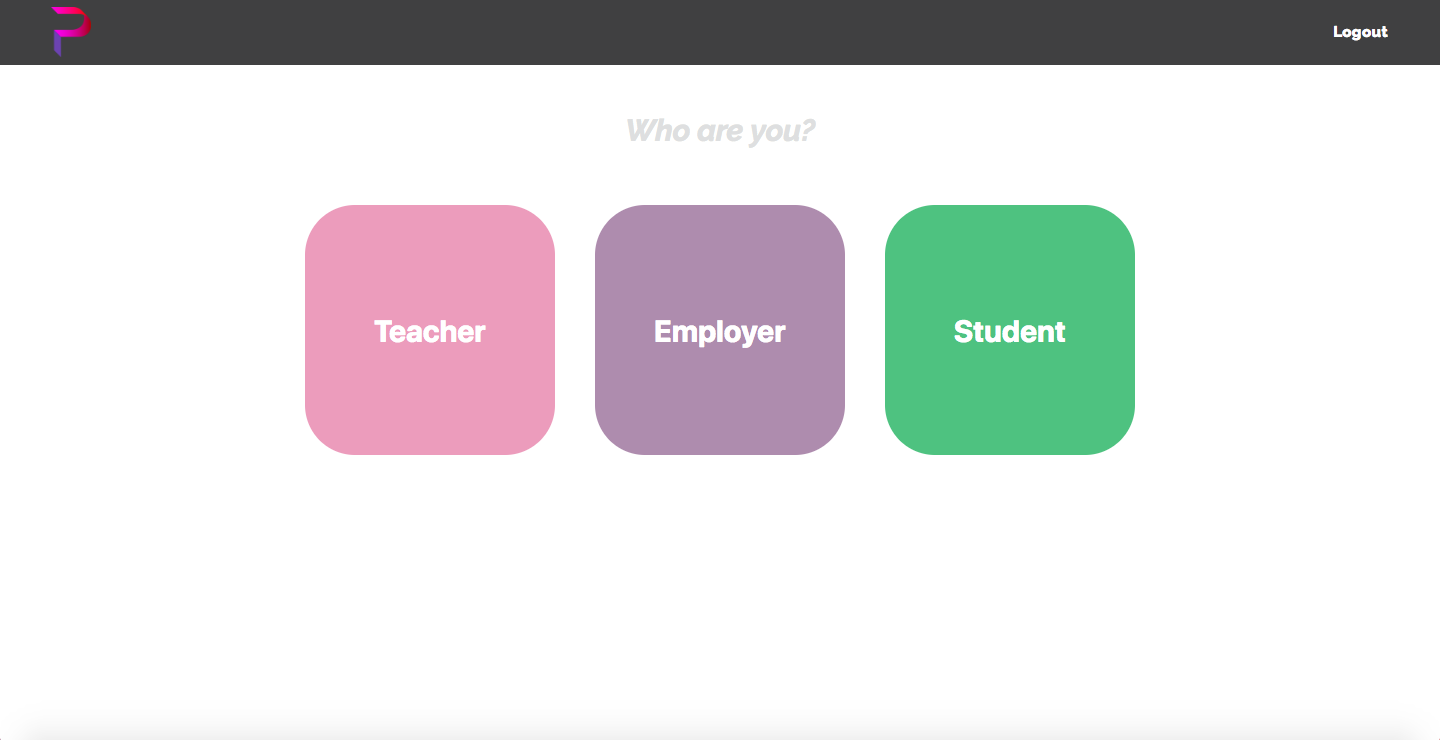
\includegraphics{type.png}}
        }\qquad\qquad
        \subfloat[][User Inputs]{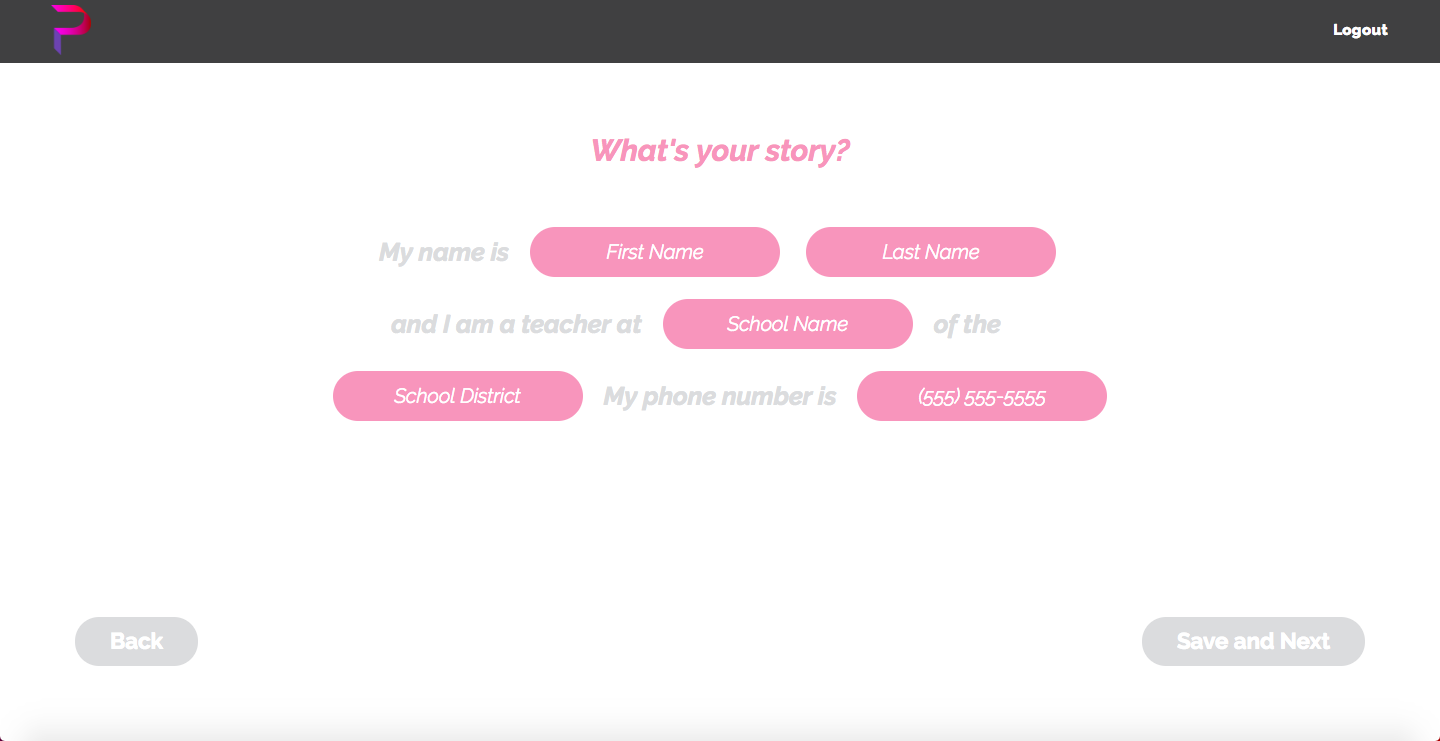
\includegraphics[scale=.26]{story.png}
        }\\
        \subfloat[][User Preferences]{\scalebox{.26}{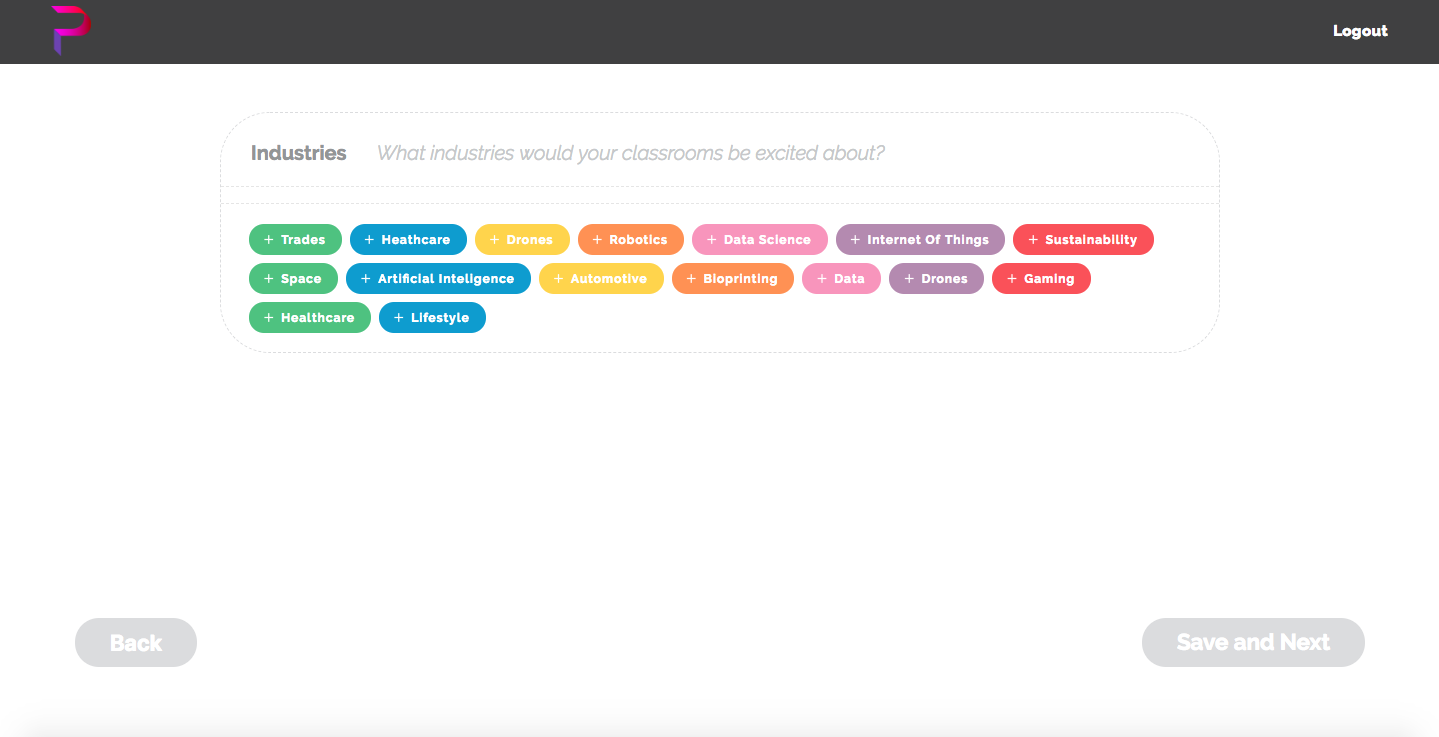
\includegraphics[origin=c]{industry.png}}
        }\qquad\qquad
        \subfloat[][Recommendations ]{\scalebox{.38}{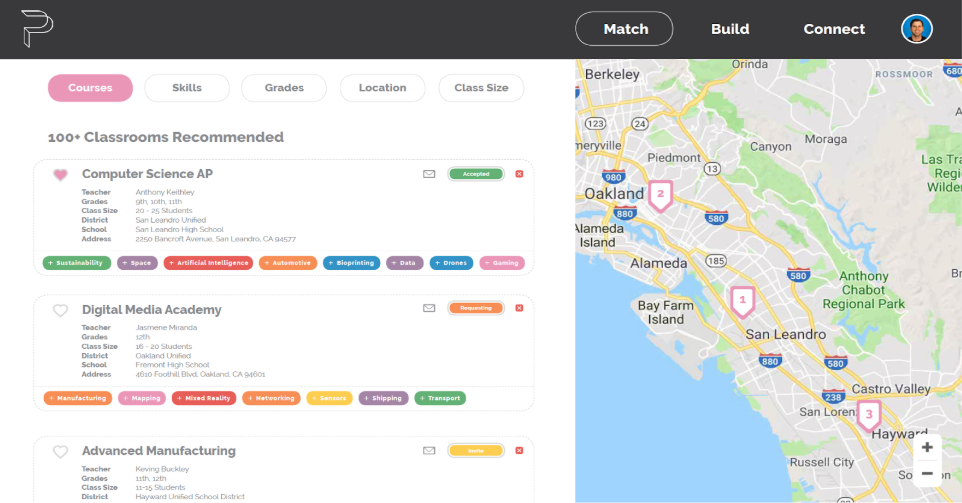
\includegraphics[origin=c]{recommender_ui.png}}
        }
  \caption[]{Onboarding web application designed based on user interviews}%
\end{figure}



\subsection{Recommender System}%

\begin{itemize}
    \item Scores compatibility between every employer and classroom
\end{itemize}
\begin{center}
\textbf{Inputs to the recommender system}
\end{center}
    \begin{itemize}
        \begin{multicols}{2}
            \centering
            \textit{Classroom}
            \vfill
            Course name, technologies, skills, industry preference
            \vfill
            \columnbreak
            \centering
            \textit{Employer} \\
            Industry, service, product, vision
        \end{multicols}
        \end{itemize}
\begin{itemize}
    \item Semantic Word Embedder: The GloVe Model
    \begin{itemize}
        \item Unsupervised learning algorithm producing vector representations of words, pre-trained on 2014 Wikipedia data
        \item Cosine distance between vectors relates to semantic similarity
    \end{itemize}
\end{itemize}

\subsection{Topic Modeling Engine}%
\begin{itemize}
    \item Built a pipeline that takes in a large corpus of texts/PDFs and returns summaries and visualizations of representative topics
    \item Experimented with algorithms such as LDA and NMF
    \item Applied these algorithms on 2000+ course syllabi scraped from Las Positas College in Livermore, CA
\end{itemize}

\begin{center}
\begin{figure}
    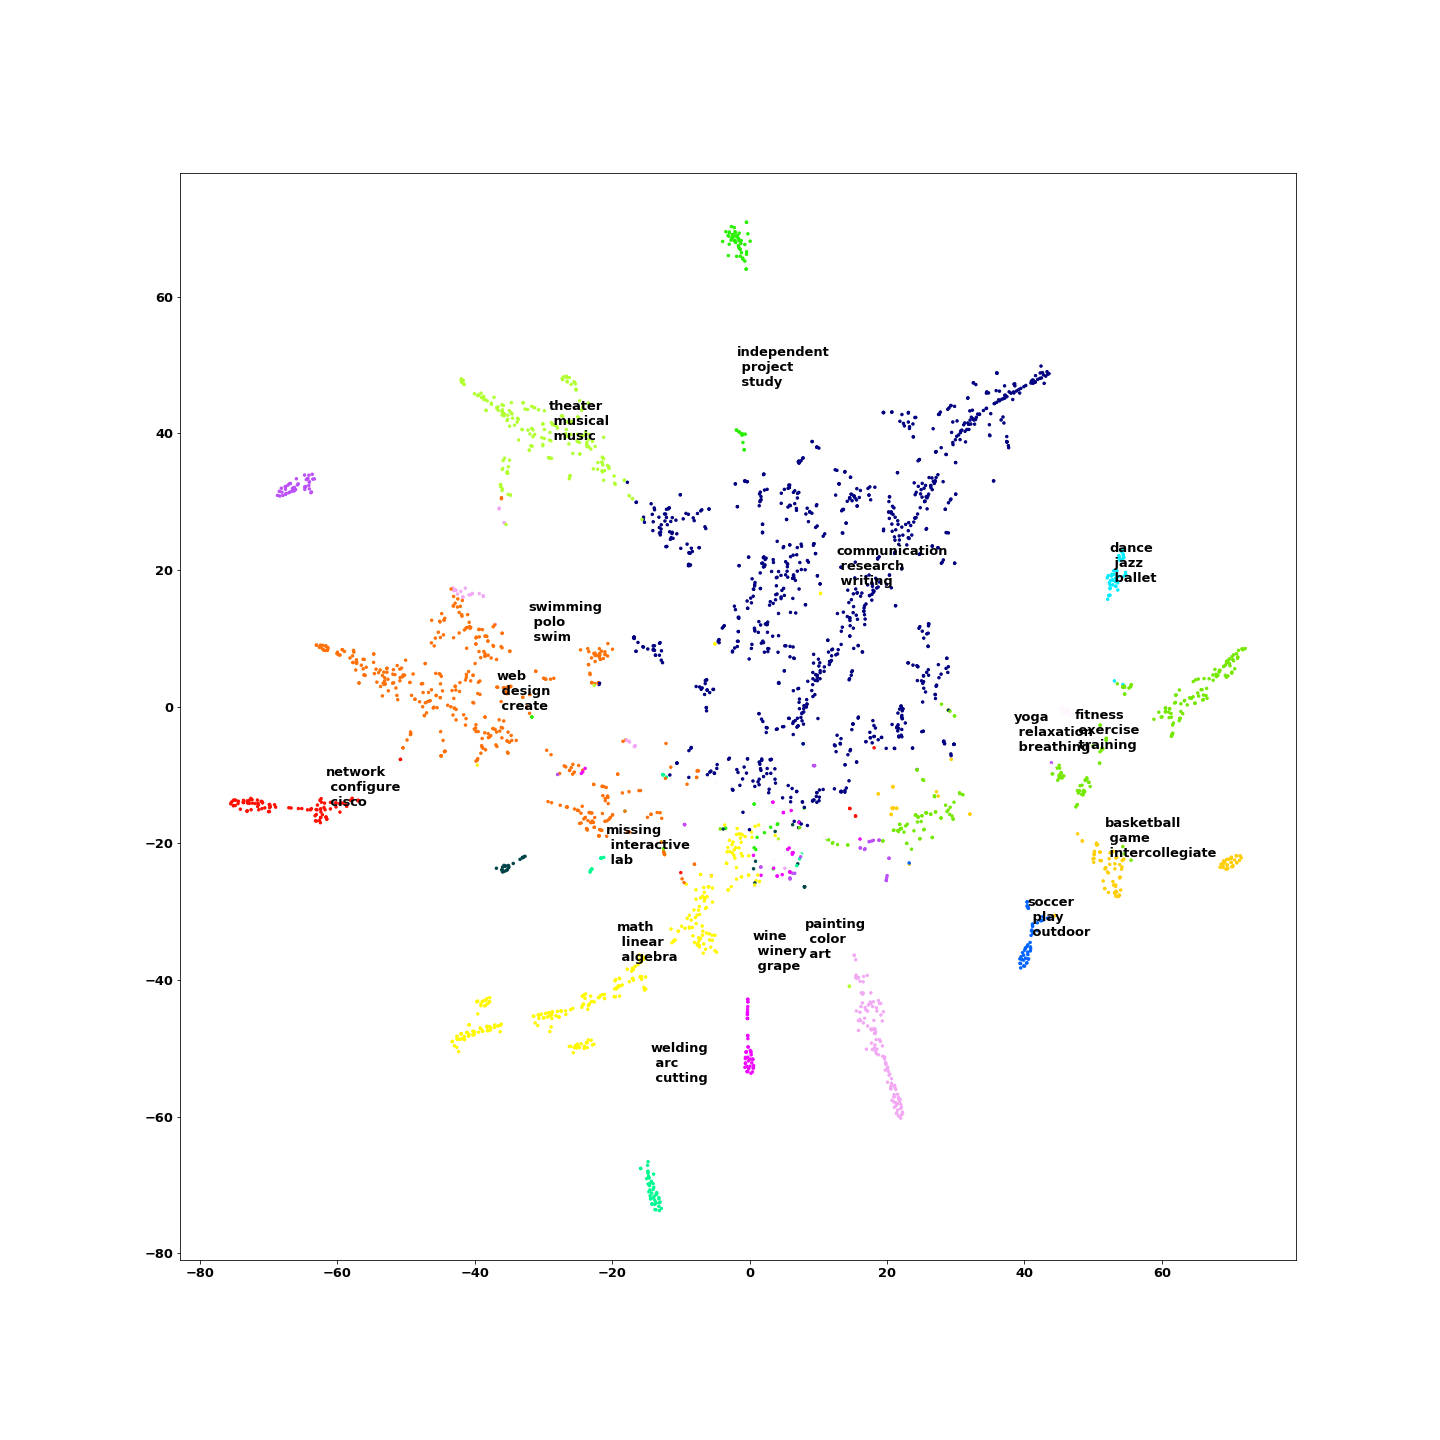
\includegraphics[scale = 0.66]{nmf_16.png}
       \caption[]{Visualization of All Las Positas Syllabi with 16 Topics using NMF}%
\end{figure}
\end{center}




% \vfill
% \columnbreak

\section{Conclusions}

% Rather than just a summary of your findings (which you presented in
% the previous section), write your \emph{conclusions} based on those
% results---what have you learned, and what does what you've learned
% mean for your reader, the world at large, and your future research?
\begin{itemize}
    \item We can extract educational priorities using a variety of NLP techniques.
    \item Our work can help institutions make data-driven decisions.
    \item Topic modeling can help improve PilotCity recommendations.
\end{itemize}

\section{For Further Information}

\begin{itemize}
\item Contact us at \url{mathclinic-pilotcity-l@g.hmc.edu}.
\item View our code at:  \url{www.github.com/hmcmathclinic/18-19-PilotCity-Code}.
\end{itemize}

\section{References}
{\small 
\begin{itemize}
    \item Greene, Derek. “Parameter Selection for NMF.” GitHub, 27 Sept. 2017.
    \item Jeffrey Pennington, Richard Socher, and Christopher D. Manning. "GloVe: Global Vectors for Word Representation." 2014. 
    \item Las Positas College. “Las Positas College CurricUNET.” 2019.
    \item Pedregosa et al. Scikit-learn: Machine Learning in Python, JMLR 12, 2011.
    \item Radim Rehurek and Petr Sojka. "Software Framework for Topic Modelling with Large Corpora." 2010.
    \item W, Shuai. “Topic Modeling and t-SNE Visualization.” Shuai's AI & Data Blog, 2016.
\end{itemize}
}

%% References.
%% Note that BibTeX will add its own section-level header, ``References''.

\bibliographystyle{hmcmath}
\bibliography{sampleposter}


\section{Acknowledgments}
We greatly appreciate Derick Lee, the PilotCity local team, Dr. Talithia Williams, Dr. Weiqing Gu, and IES for supporting our project.

\subsection{Team Members}
\begin{multicols}{2}
\setlength{\columnseprule}{0pt}
Madison Hobbs (PM), Aanya Alwani, Dominique Macias, Jean Adedze, Xuming Liang
\vfill
\columnbreak
\textbf{Faculty Advisor} Dr. Talithia Williams \\
\textbf{Liaison} Derick Lee, PilotCity
\end{multicols}


\vfill


\end{poster}

\end{document}

 
